\documentclass[handout]{beamer}
% \documentclass{beamer}

%%
%%
%%
% From http://tex.stackexchange.com/questions/2072/beamer-navigation-circles-without-subsections
% Solution #2 or 3:
% \usepackage{etoolbox}
% \makeatletter
% % replace the subsection number test with a test that always returns true
% \patchcmd{\slideentry}{\ifnum#2>0}{\ifnum2>0}{}{\@error{unable to patch}}%
% \makeatother
% Solution #1:
\usepackage{remreset}% tiny package containing just the \@removefromreset command
\makeatletter
\@removefromreset{subsection}{section}
\makeatother
\setcounter{subsection}{1}


\usepackage{etex}
\usepackage{pgf}
\usepackage{tikz}
\usepackage{url}
\usepackage{amsmath}
\usepackage{color}
% \definecolor{red}{rgb}{1,0,0}
\usepackage{ulem}
% \usepackage{booktabs}
\usepackage{colortbl,booktabs}
\renewcommand*{\thefootnote}{\fnsymbol{footnote}}
\usepackage{fancybox}
\usepackage[framemethod=TikZ]{mdframed}
\mdfdefinestyle{FactStyle}{%
  outerlinewidth=0.5,
  roundcorner=1pt,
  leftmargin=1cm,
  linecolor=blue,
  outerlinecolor=blue!70!black,
  backgroundcolor=yellow!40
}
\usepackage{cancel}

  \newcommand\Warning{%
    \makebox[2.4em][c]{%
      \makebox[0pt][c]{\raisebox{.2em}{\Large!}}%
      \makebox[0pt][c]{\color{red}\Huge$\bigtriangleup$}}}%

\usepackage{stackengine}
\usepackage{scalerel}
\usepackage{xcolor}
  \newcommand\dangersign[1][2ex]{%
    \renewcommand\stacktype{L}%
    \scaleto{\stackon[1.3pt]{\color{red}$\triangle$}{\tiny !}}{#1}%
  }



\usepackage{dcolumn}
\newcolumntype{d}[1]{D{.}{.}{#1}}

% From
% http://tex.stackexchange.com/questions/109900/how-can-i-box-multiple-aligned-equations
\usepackage{empheq}
\usepackage{tcolorbox}  \newtcbox{\othermathbox}[1][]{%
  nobeforeafter, tcbox raise base, 
  colback=black!10, colframe=red!30, 
  left=1em, top=0.5em, right=1em, bottom=0.5em}

\newcommand\blue{\color{blue}}
\newcommand\red{\color{red}}
\newcommand\green{\color{green!75!black}}
\newcommand\purple{\color{purple}}
\newcommand\bluegreen{\color{blue!75!green}}
\newcommand\orange{\color{orange}}
\newcommand\redgreen{\color{red!50!green}}
\newcommand\grey{\color{black}}
\newcommand\gap{\vspace{.1in}}
\newcommand\nb{${\red\bullet}\ $}
\newcommand\halfgap{\vspace{.05in}}
\newcommand\divideline{\line(1,0){352}}
\usepackage{marvosym} % for \Smiley

\newcommand{\bluealert}[1]{{\blue\textbf{#1}}}

% \usepackage{beamerthemesplit} %Key package for beamer
\usetheme{Singapore}
% \usetheme{Szeged}
% \usetheme{Garfield}
% \usetheme{CambridgeUS}
% \usenavigationsymbolstemplate{} %Gets rid of slide navigation symbols


\setbeamercolor{separation line}{use=structure,bg=structure.fg!50!bg}
% \begin{beamercolorbox}[colsep=0.5pt]
%   {upper separation line foot}
% \end{beamercolorbox}



\makeatletter
\setbeamertemplate{footline}
{
  \leavevmode%
  \hbox{%
% \begin{beamercolorbox}[colsep=0.5pt]
%   {upper separation line foot}
% \end{beamercolorbox}


  \begin{beamercolorbox}[wd=.5\paperwidth,ht=2.25ex,dp=2ex,colsep=0.5pt]%
    {upper separation line foot}
    \usebeamerfont{author in head/foot}%
    \hspace*{2ex}\insertshortdate:\ \insertshorttitle
  \end{beamercolorbox}%
  \begin{beamercolorbox}[wd=.5\paperwidth,ht=2.25ex,dp=2ex,right]{title in head/foot}%
    \usebeamerfont{title in head/foot}
    {\insertshortauthor}\hspace*{2ex}
  \end{beamercolorbox}}%
  % \begin{beamercolorbox}[wd=.333333\paperwidth,ht=2.25ex,dp=2ex,right]{date in head/foot}%
  %   \usebeamerfont{date in head/foot}\insertshortdate{}\hspace*{2em}
  %   \insertframenumber{} / \inserttotalframenumber\hspace*{2ex} 
  % \end{beamercolorbox}%
  \vskip0pt%
}
\makeatother

\usetikzlibrary{decorations.markings}
\usetikzlibrary{arrows}


\title{Final Exam Review}
\author{Peter Garfield, UCSB Mathematics}
\date{March 15, 2017}
%\institute{}


\useinnertheme{default}

\usefonttheme{serif}
% \usecolortheme{rose}
% \usecolortheme{whale}
% \usecolortheme{orchid}
\usecolortheme{crane}
% \usecolortheme{dolphin}


%TEMPLATE
\setbeamertemplate{navigation symbols}{}

\setbeamertemplate{note page}[compress]

\setbeamertemplate{frametitle}{
  \vspace{0.5em}
  % \begin{centering}
  {\huge\blue\textbf{\textmd{\insertframetitle}}}
  \par
  % \end{centering}
}

% From http://tex.stackexchange.com/questions/7032/good-way-to-make-textcircled-numbers:
\newcommand*\circled[1]{\tikz[baseline=(char.base)]{\node[shape=circle,draw,fill=orange,inner sep=1pt] (char) {#1};}} 
% \renewcommand{\labelenumi}{\circled{\textbf{\arabic{enumi}}}}

\let\olddescription\description
\let\oldenddescription\enddescription
\usepackage{enumitem}
\let\description\olddescription
\let\enddescription\oldenddescription

% \usepackage[loadonly]{enumitem}
\setlist[enumerate,1]{label=\colorbox{orange}{\arabic*.},font=\bfseries}
%\setlist[enumerate,2]{label=\colorbox{blue!25}{(\alph*)},font=\bfseries}
% \setlist[enumerate,1]{label=\arabic*.,font=\bfseries}
\setlist[itemize,1]{label=\red$\bullet$}
\setlist[itemize,2]{label=\blue$\bullet$}

\newcommand\answer[1]{\fbox{#1}}
% \renewcommand\answer[1]{}

\newcommand{\antilog}{\operatorname{antilog}}







\title{}
\title{Concavity \& Second Derivatives}
\date{May 24, 2017}


\begin{document}
\small

\section*{Administration}

\frame{
  \frametitle{Office Hours!}
  % \ \vspace*{0.25in}

  {\Large{}Instructor:}\\
  \ \hspace*{0.2in} Trevor Klar, \url{trevorklar@math.ucsb.edu}\\[0.25em]

  {\Large{}Office Hours:}\\
  \ \hspace*{0.2in} Mondays 2--3\textsc{pm}\\
  \ \hspace*{0.2in} Tuesdays 10:30--11:30\textsc{am}\\
  \ \hspace*{0.2in} Thursdays 1--2\textsc{pm}\\
  \ \hspace*{0.2in} or by appointment \\[0.25em]

  {\Large{}Office:}\\
  \ \hspace*{0.2in} South Hall 6431X (Grad Tower, 6th floor, blue side, first door on the right)\\[0.5em]

  \copyright\ 2017\ Daryl Cooper, Trevor Klar

  % \vspace*{2in}
}


\section{Higher Derivatives}

\frame{
  \frametitle{\S8.12: The Second Derivative}

  \alert{Today:}\ We can take the derivative of a function repeatedly!
  \bigskip

  \alert{Example:}\ If $f(x)=x^3-3x+2$, then
  \begin{itemize}
  \item[\nb] $\dfrac{df}{dx}={\blue f'(x)}= $ \pause ${\blue 3x^2-3}$
    \smallskip

  \item[\nb] The {\red second derivative} of $f(x)$ is $\displaystyle
      \frac{d}{dx}\left(\frac{df}{dx}\right)
      = {\red f''(x)}
      = 
      \pause 
      {\red 6x}$.
    \pause\newline
    This is written $f''(x)$ or $\dfrac{d^2f}{dx^2}$.
    \pause

  \item[\nb] The {\red
      third derivative} of $f(x)$ is $\displaystyle
      \frac{d}{dx}\left(\frac{d^2f}{dx^2}\right)
      = {\red f'''(x)}
      = 
      \pause 
      {\red 6}$.
    \pause\newline
    This is written $f'''(x)$ or $\dfrac{d^3f}{dx^3}$.
    \pause

  \item[\nb] {\blue Keep Going!}\ \ \pause 
    The {\red fourth derivative}\ is $\dfrac{d^4f}{dx^4} = f''''(x) =
    0$. 
    \pause

  \item[\nb]
    The fun ends here, for this $f(x)$ all {\red higher derivatives} are zero.
  \end{itemize}

}

\frame{
  \frametitle{Examples}

  General idea: Differentiating the function ${\red n}$ times gives us
  the {\blue ${\red n}$th derivative} of $f$.  
  It is written as
  \begin{equation*}
    {{f'''}^{\cdots}}{}''''(x) 
    = f^{(n)}(x)
    = \frac{d^nf}{dx^n}.
  \end{equation*}
  \bigskip
  \pause

  {\red(1)}\ What is the second derivative of $3x^2-5x+7$?
  \begin{center}
    A$=0$
    \quad 
    B$ = 7$
    \quad 
    C$ = 6$
    \quad 
    D$ = 3$
    \quad 
    E$ = -5$
    \pause
    \quad
    \fbox{C}
  \end{center}
  \bigskip
  \pause

  {\red(2)}\ $\dfrac{d^2}{dx^2}\left(x^5\right)=$?
  \begin{center}
    A$ = 20$
    \quad 
    B$ = 5x^4$
    \quad 
    C$ = 0$
    \quad 
    D$ = 20x^4$
    \quad 
    E$ = 20x^3$
    \pause
    \quad
    \fbox{E}
  \end{center}
  \bigskip
  \pause

  {\red(3)}\ $\dfrac{d^2}{dx^2}\left(\sqrt{x}\right)=$?
  \begin{center}
    A$ = \frac{1}{4}x^{-3/2}$
    \quad 
    B$ = \frac{-1}{4}x^{-1/2}$
    \quad 
    C$ = \frac{-1}{4}x^{-3/2}$ 
    \quad 
    D$ = \frac{1}{2}x^{-1/2}$
    \quad 
    E$ = 0$
    \pause
    \ 
    \fbox{C}
  \end{center}

}



\frame{
  \frametitle{More Examples}

  {\red(4)}\ $\dfrac{d^2}{dt^2}\left(e^{{\red 3}t}\right)=$?
  \begin{center}
    A$ = e^{3t}$
    \quad 
    B$ = 3e^{2t}$
    \quad 
    C$ = 9e^{3t}$
    \quad 
    D$ = 3e^{3t}$
    \quad 
    E$ = 9e^t$
    \pause
    \qquad
    \fbox{C}
  \end{center}
  \gap 

  {\red(5)} Find $f{\red '''}(x)$ when $f(x)=x^3$.
  \begin{center}
    A$=  6x^2$
    \quad 
    B$ = 0$
    \quad 
    C$ = 3x$
    \quad 
    D$ = 3x^2$
    \quad 
    E$ = 6$
    \pause
    \quad
    \fbox{E}
  \end{center}
  \bigskip

  {\red(6)}\ If $f(x)= x^3-4x^2 + 7x -31$, then $f{\red ''}(10)=$? 
  \begin{center}
    A$ = 6$
    \quad 
    B$ = 3x^2-8x$
    \quad 
    C$ = 6x$
    \quad 
    D$ = 60$
    \quad 
    E$ = 52$
    \pause
    \quad
    \fbox{E}
  \end{center}
  \bigskip


}


\section{Acceleration}

\frame{
  \frametitle{Example: Acceleration}

  The {\red acceleration}\ due to gravity is
  \begin{equation*}
    32\ \text{{\blue feet per second per second}}
      = 32\ \text{ft}/\text{sec}^2. 
  \end{equation*}
  \vspace*{-1em}

  \uncover<2->{%
    \bluealert{This means:}
    \begin{center}
      \begin{mdframed}[style=FactStyle]
        every second you fall, \\
        your speed increases by $32\ \text{ft}/\text{sec}$
        \uncover<3->{$\approx 22\ \text{mph}$.}
        % \vspace*{-1em}
      \end{mdframed}
    \end{center}
  }
  \begin{align*}
    \uncover<4->{%
    \text{{\red acceleration}}
    & = \text{{\orange rate of change}\ of {\blue velocity}} 
    & = \text{{\orange derivative} of {\blue velocity}}.\\
    }
    \uncover<5->{%
    \text{{\blue velocity}}
    & = \text{{\orange rate of change} of {\purple distance}}
    & = \text{{\orange derivative} of {\purple distance}}.
      }
  \end{align*}

  \uncover<6->{%
    Therefore
    \begin{center}
      \begin{mdframed}[style=FactStyle]
        \vspace*{-0.5em}
        \begin{equation*}
          \text{{\red acceleration}}
          = \text{second derivative of {\purple distance}}
        \end{equation*}
      \end{mdframed}
    \end{center}
  }

  \uncover<7->{%
    \alert{Example:}\ Height of ball is $h(t)=20t-5t^2$\ meters after $t$ seconds.\\
    {\red (a)}\ {\blue Velocity}\ of ball after $t$ seconds is\ 
  }
  \uncover<8->{$h{\red '}(t)=20-10t\ \text{m}/\text{sec}$}\\
  \uncover<9->{%
    {\red (b)}\ {\red Acceleration}\ of ball after $t$ seconds is\ 
  }
  \uncover<10->{$h{\red''}(t)=-10\ \text{m}/\text{sec}^2$}

  % \gap $\purple -$ sign because UP is positive in this problem and gravity accelerates DOWN so acceleration is {\purple negative}

}

\frame{
  \frametitle{It's not the speed that kills}
  % \includegraphics[scale=0.7]{speedkills.pdf}
  % \gap 

  Suppose you hit a brick wall at $60$ mph.
  \pause

  \alert{Question:}\ What is your (sudden!) acceleration?
  \pause

  \begin{align*}
    \left( \ \parbox{1.08in}{%
    \ Average rate of\ \\
    change of velocity\\
    \hspace*{0.2in}in stopping 
    }\ 
    \right)
    & = \frac{\Delta\ \text{velocity}}{\Delta\ \text{time}}
      = \frac{-60\ \text{mph}}{1/10\ \text{sec}} \\
    & \approx \frac{-88\ \text{ft}/\text{sec}}{1/10\ \text{sec}}
      = -880\ \text{ft}/\text{sec}^2.
  \end{align*}
  \pause
  Since $1\ \text{gravity} = 32\ \text{ft}/\text{sec}^2$, this is about
  \begin{equation*}
    880\ \text{ft}/\text{sec}^2
    = \left( 880\ \text{ft}/\text{sec}^2 \right)
    \times \frac{1\ \text{gravity}}{32\ \text{ft}/\text{sec}^2}
    \pause
    \approx 28\ \text{``g''}.
  \end{equation*}
  %
  The force which pushes you at the windshield is about {\red{}28}
  times your weight.
  \pause

  If you weigh $110$ pounds, this force is about $\text{\red $3000$\ pounds}
  = \text{\red $1.5$\ tons}$.

}


\frame{
  \frametitle{Rocket!}

  A rocket is fired vertically upwards.  The height after $t$ seconds
  is $2t^3+5t^2$ meters.
  \smallskip

  \alert{Question:}\ What is the acceleration in
  $\text{m}/\text{sec}^2$ after $t$ seconds? 
  \begin{center}
    A$=2t^3+5t^2$
    \quad 
    B$=6t^2+10t$
    \quad 
    C$ = 12t+10$
    \quad 
    D$ = 12$
    \quad 
    E$ = 0$
    \pause
    \quad
    \fbox{C}
  \end{center}
  \medskip
  \pause

  Idea:
  \begin{itemize}
  \item[\nb] $h(t) = \text{height in meters at time $t$ seconds}$ 
    \smallskip

  \item[\nb] $h'(t) = \text{velocity in $\text{m}/\text{sec}$\ at time $t$ seconds}$ 
    \smallskip

  \item[\nb] $h''(t) = \text{acceleration in $\text{m}/\text{sec}^2$\ at time $t$ seconds}$ 
    \bigskip

  \end{itemize}

  \alert{More Questions:}
  \smallskip

  {\red(a)}\ What can we say about $f(t)$ if $f'(t)=0$ for {\red all} $t$?
  \pause
  \smallskip

  {\red(b)}\ What can we say about $f(t)$ if $f''(t)=0$ for {\red all} $t$?
  \pause
  \smallskip

  \vspace*{2in}

}

\section{Concavity}

\frame{
  \frametitle{Application 2: Concavity}

  \begin{align*}
    \frac{df}{dx}
    & = \text{rate of change of $f(x)$}\\[0.5em]
    %
    \text{and so}\ 
    \frac{d^2f}{dx^2}
    & =\frac{d}{dx}\left({\red \frac{df}{dx}}\right)
      = \text{rate of change of $\red\dfrac{df}{dx}$}
  \end{align*}

  \bluealert{Conclusion:}\\[-2em]
  \begin{center}
    \begin{mdframed}[style=FactStyle]
      The second derivative tells you how quickly the {\red rate of
        change} is changing.
    \end{mdframed}
  \end{center}
  \vspace*{-1em}

  \bluealert{Uses of second derivative:}
  \begin{itemize}
  \item[\nb] We've seen: {\blue acceleration} is the rate of change of velocity \\
    So: {\blue acceleration}\ is the second derivative of distance traveled.
    \pause

  \item[\nb] Is the graph {\blue concave up} or {\blue concave down}?
    \pause

  \item[\nb] Are things  {\blue changing for better or worse}?

  \end{itemize}

}

\frame{
  \frametitle{Meanings: The First Derivative}

  \begin{center}
    \begin{tikzpicture}[x=15mm,y=5mm,>=latex]
      \only<1>{%
        \draw[ultra thick,blue,domain=-1:3,smooth] plot (\x,{(\x)^3-3*(\x)^2+2});
      }
      \only<2->{%
        \draw[ultra thick,blue,domain=-1:0,smooth] plot (\x,{(\x)^3-3*(\x)^2+2});
        \draw[ultra thick,red,domain=0:2,smooth] plot (\x,{(\x)^3-3*(\x)^2+2});
        \draw[ultra thick,blue,domain=2:3,smooth] plot (\x,{(\x)^3-3*(\x)^2+2});
        \filldraw[green] (0,2) circle (2pt);
        \filldraw[green] (2,-2) circle (2pt);
      }
      \uncover<3->{%
        \draw[ultra thick,blue,<-] (-1,-2.5) -- (0,-2.5);
        \draw[blue,fill=white] (0,-2.5) circle (2pt);
        \draw[ultra thick,blue,->] (2,-2.5) -- (3,-2.5);
        \draw[blue,fill=white] (2,-2.5) circle (2pt);
        \draw[ultra thick,red] (0,-2.85) -- (2,-2.85);
        \draw[red,fill=white] (0,-2.85) circle (2pt);
        \draw[red,fill=white] (2,-2.85) circle (2pt);
        \node[blue] at (-0.5,-3.5) {$f(x)$ incr};
        \node[red] at (1,-3.5) {$f(x)$\ decr};
        \node[blue] at (2.5,-3.5) {$f(x)$\ incr};
      }
      \uncover<5->{%
        \node[blue] at (-0.5,-4.5) {$f'(x)>0$};
        \node[red] at (1,-4.5) {$f'(x)<0$};
        \node[blue] at (2.5,-4.5) {$f'(x)>0$};
      }
      \begin{scope}
        \clip (-1.5,-4) rectangle (3.5,2.75);
              \uncover<4->{%
        % Tangent lines to $y=x^3-3x^2+2$ has slope $y'=3x^2-6x=3x(x-2)$.
        % \draw[blue,domain=-1:0] plot (\x,{(-5/5)^3-3*(-5/5)^2+2+3*(-5/5)*(-5/5-2)*(\x+5/5)});
        % \draw[blue,domain=-1:0] plot (\x,{(-4/5)^3-3*(-4/5)^2+2+3*(-4/5)*(-4/5-2)*(\x+4/5)});
        % \draw[blue,domain=-1:0] plot (\x,{(-3/5)^3-3*(-3/5)^2+2+3*(-3/5)*(-3/5-2)*(\x+3/5)});
        % \draw[blue,domain=-1:0] plot (\x,{(-2/5)^3-3*(-1/5)^2+2+3*(-2/5)*(-2/5-2)*(\x+2/5)});
        % \draw[blue,domain=-1:0] plot (\x,{(-1/5)^3-3*(-1/5)^2+2+3*(-2/5)*(-1/5-2)*(\x+1/5)});
        % \draw[blue,domain=-1:0] plot (\x,{(-1/3)^3-3*(-1/3)^2+2+3*(-1/3)*(-1/3-2)*(\x+1/3)});
        \draw[thick,blue,domain=-1:0] plot (\x,{(-1/2)^3-3*(-1/2)^2+2+3*(-1/2)*(-1/2-2)*(\x+1/2)});
        \draw[thick,red,domain=0:1.85] plot (\x,{(1)^3-3*(1)^2+2+3*(1)*(1-2)*(\x-1)});
        \draw[thick,blue,domain=2.2:3.5] plot (\x,{(2.5)^3-3*(2.5)^2+2+3*(2.5)*(2.5-2)*(\x-2.5)});
        \fill[black] (-0.5,{(-1/2)^3-3*(-1/2)^2+2}) circle (2pt);
        \fill[black] (1,{(1)^3-3*(1)^2+2}) circle (2pt);
        \fill[black] (2.5,{(2.5)^3-3*(2.5)^2+2}) circle (2pt);
      }
      \end{scope}
    \end{tikzpicture}
  \end{center}
  \bigskip

  \uncover<6->{%
    \bluealert{Point:} 

    \begin{mdframed}[style=FactStyle]
      \vspace*{-1.25em}
      \begin{align*}
        {\blue f'(x) > 0} & \iff\ \text{$f(x)$\ is increasing} \\
        {\red f'(x) < 0} & \iff\ \text{$f(x)$\ is decreasing} 
      \end{align*}
    \end{mdframed}
  }
  \vspace*{3in}

}

\frame{
  \frametitle{Meanings: The Second Derivative}

  \begin{center}
    \begin{tikzpicture}[x=15mm,y=5mm,>=latex]
      \only<1>{%
        \draw[ultra thick,blue,domain=-1:3,smooth] plot (\x,{(\x)^3-3*(\x)^2+2});
      }
      \only<2->{%
        \draw[ultra thick,green!50!black,domain=-1:1,smooth] plot (\x,{(\x)^3-3*(\x)^2+2});
        \draw[ultra thick,orange!90!black,domain=1:3,smooth] plot (\x,{(\x)^3-3*(\x)^2+2});
        \filldraw[blue] (1,0) circle (2pt);
      }
      \uncover<3->{%
        \draw[ultra thick,green!50!black,<-] (-1,-2.5) -- (1,-2.5);
        \draw[green!50!black,fill=white] (1,-2.5) circle (2pt);
        \draw[ultra thick,orange!90!black,->] (1,-2.85) -- (3,-2.85);
        \draw[orange!90!black,fill=white] (1,-2.85) circle (2pt);
        \node[green!50!black] at (0,-3.5) {$f(x)$ cc down};
        \node[orange!90!black] at (2,-3.5) {$f(x)$\ cc up};
      }
      \begin{scope}
        \clip (-1.5,-4) rectangle (3.5,2.75);
              \uncover<4->{%
        % Tangent lines to $y=x^3-3x^2+2$ has slope $y'=3x^2-6x=3x(x-2)$.
        % \draw[blue,domain=-1:0] plot (\x,{(-5/5)^3-3*(-5/5)^2+2+3*(-5/5)*(-5/5-2)*(\x+5/5)});
        % \draw[blue,domain=-1:0] plot (\x,{(-4/5)^3-3*(-4/5)^2+2+3*(-4/5)*(-4/5-2)*(\x+4/5)});
        % \draw[blue,domain=-1:0] plot (\x,{(-3/5)^3-3*(-3/5)^2+2+3*(-3/5)*(-3/5-2)*(\x+3/5)});
        % \draw[blue,domain=-1:0] plot (\x,{(-2/5)^3-3*(-1/5)^2+2+3*(-2/5)*(-2/5-2)*(\x+2/5)});
        % \draw[blue,domain=-1:0] plot (\x,{(-1/5)^3-3*(-1/5)^2+2+3*(-2/5)*(-1/5-2)*(\x+1/5)});
        % \draw[blue,domain=-1:0] plot (\x,{(-1/3)^3-3*(-1/3)^2+2+3*(-1/3)*(-1/3-2)*(\x+1/3)});
        \draw[thick,green!50!black,domain=-1:0] plot (\x,{(-2/3)^3-3*(-2/3)^2+2+3*(-2/3)*(-2/3-2)*(\x+2/3)});
        \draw[thick,green!50!black,domain=-1:0.3333] plot (\x,{(-1/3)^3-3*(-1/3)^2+2+3*(-1/3)*(-1/3-2)*(\x+1/3)});
        \draw[thick,green!50!black] (-0.5,2) -- (0.5,2);
        \draw[thick,green!50!black,domain=-0.3333:1] plot (\x,{(1/3)^3-3*(1/3)^2+2+3*(1/3)*(1/3-2)*(\x-1/3)});
        \draw[thick,green!50!black,domain=0:1] plot (\x,{(2/3)^3-3*(2/3)^2+2+3*(2/3)*(2/3-2)*(\x-2/3)});
        % \draw[thick,red,domain=0:1.85] plot (\x,{(1)^3-3*(1)^2+2+3*(1)*(1-2)*(\x-1)});
        % \draw[thick,blue,domain=2.2:3.5] plot (\x,{(2.5)^3-3*(2.5)^2+2+3*(2.5)*(2.5-2)*(\x-2.5)});
        \fill[black] ({-2/3},{(-2/3)^3-3*(-2/3)^2+2}) circle (2pt);
        \fill[black] ({-1/3},{(-1/3)^3-3*(-1/3)^2+2}) circle (2pt);
        \fill[black] (0,2) circle (2pt);
        \fill[black] ({1/3},{(1/3)^3-3*(1/3)^2+2}) circle (2pt);
        \fill[black] ({2/3},{(2/3)^3-3*(2/3)^2+2}) circle (2pt);
        % \fill[black] (1,{(1)^3-3*(1)^2+2}) circle (2pt);
        % \fill[black] (2.5,{(2.5)^3-3*(2.5)^2+2}) circle (2pt);
      }
      \uncover<6->{%
        \draw[thick,orange!90!black,domain=2.3:3.3] plot (\x,{(8/3)^3-3*(8/3)^2+2+3*(8/3)*(8/3-2)*(\x-8/3)});
        \draw[thick,orange!90!black,domain=1.9:2.9] plot (\x,{(7/3)^3-3*(7/3)^2+2+3*(7/3)*(7/3-2)*(\x-7/3)});
        \draw[thick,orange!90!black] (1.5,-2) -- (2.5,-2);
        \draw[thick,orange!90!black,domain=1.3333:2.1] plot (\x,{(5/3)^3-3*(5/3)^2+2+3*(5/3)*(5/3-2)*(\x-5/3)});
        \draw[thick,orange!90!black,domain=0.5:2] plot (\x,{(4/3)^3-3*(4/3)^2+2+3*(4/3)*(4/3-2)*(\x-4/3)});
        % \draw[thick,red,domain=0:1.85] plot (\x,{(1)^3-3*(1)^2+2+3*(1)*(1-2)*(\x-1)});
        % \draw[thick,blue,domain=2.2:3.5] plot (\x,{(2.5)^3-3*(2.5)^2+2+3*(2.5)*(2.5-2)*(\x-2.5)});
        \fill[black] ({4/3},{(4/3)^3-3*(4/3)^2+2}) circle (2pt);
        \fill[black] ({5/3},{(5/3)^3-3*(5/3)^2+2}) circle (2pt);
        \fill[black] (2,-2) circle (2pt);
        \fill[black] ({7/3},{(7/3)^3-3*(7/3)^2+2}) circle (2pt);
        \fill[black] ({8/3},{(8/3)^3-3*(8/3)^2+2}) circle (2pt);
      }
      \end{scope}
      \uncover<5->{%
        \node[green!50!black] at (0,-4.5) {$f''(x)<0$};
      }
      \uncover<7->{%
        \node[orange!90!black] at (2,-4.5) {$f''(x)>0$};
      }
    \end{tikzpicture}
  \end{center}
  \vspace*{-1em}

  \uncover<8->{%
    \bluealert{Point:} 

    \begin{mdframed}[style=FactStyle]
      \vspace*{-1.25em}
      \begin{align*}
        {\color{orange!90!black}f''(x) > 0} 
        & \iff\ \text{$f'(x)$\ is increasing} \\
        & \iff\ \text{$f(x)$\ is concave up} \\[0.5em]
        {\color{green!50!black}f''(x) < 0}
        & \iff\ \text{$f'(x)$\ is decreasing} \\
        & \iff\ \text{$f(x)$\ is concave down} 
      \end{align*}
    \end{mdframed}
  }
  \vspace*{3in}

}



\frame{
  \frametitle{Concavity}

  \begin{mdframed}[style=FactStyle]
    \vspace*{-1.25em}
    \begin{align*}
      {\color{orange!90!black}f''(x) > 0} & \iff\ \text{$f(x)$\ is concave up} \\
      {\color{green!50!black}f''(x) < 0} & \iff\ \text{$f(x)$\ is concave down} 
    \end{align*}
  \end{mdframed}

  {\red(1)}\ For which values of $x$ is $f(x)=x^3-6x^2+3x+2$ concave up?
  \begin{center}
    A\ when $x=0$
    \quad 
    B\ when $x<6$
    \quad 
    C\ when $x>6$\\
    \ 
    \quad 
    D\ when $x<2$
    \quad 
    E\ when $x>2$
    \quad
    \uncover<2->{\fbox{E}}
  \end{center}

  \uncover<3->{
  {\red(2)}\ Where is $f{\red''}(x)>0$? 

  \
  \hfill
  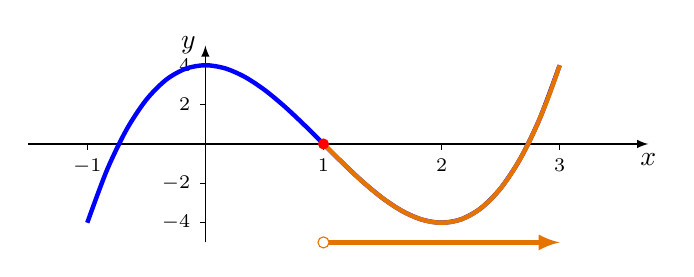
\begin{tikzpicture}[x=15mm,y=2.5mm,>=latex]
    %
    \draw[thin,black,->] (-1.5,0) -- (3.75,0) node[below] {$x$};
    \draw[thin,black,->] (0,-5) -- (0,5) node[left] {$y$};
    % ticks:
    \foreach \x in {-1,1,2,3}
    {
      \draw[thin,black] (\x,0) -- (\x,-2pt) node[below] {$\scriptstyle\x$};
    }
    \foreach \y in {-4,-2,2,4}
    {
      \draw[thin,black] (0,\y) -- (-2pt,\y) node[left] {$\scriptstyle\y$};
    }
    \draw[ultra thick,blue,domain=-1:3,smooth] plot (\x,{2*(\x)^3-6*(\x)^2+4});
    \uncover<4->{%
      \draw[ultra thick,orange!90!black,domain=1:3,smooth] plot (\x,{2*(\x)^3-6*(\x)^2+4});
      \draw[ultra thick,orange!90!black,->] (1,-5) -- (3,-5);
      \draw[orange!90!black,fill=white] (1,-5) circle (2pt);
      \fill[red] (1,0) circle (2pt);
    }
  \end{tikzpicture}
  \hfill
  \ 
  \vspace*{-1em}

  \begin{center}
    A\ when $x<2$
    \quad 
    B\ when $x>2$
    \quad
    C\ when $x<1$\\
    \ 
    \quad 
    D\ when $x>1$
    \quad
    E\ when $-0.7<x<1$
    \pause
    \quad
    \uncover<4->{\fbox{D}}
  \end{center}
}

}

\section{Review Problems}

\frame{ \frametitle{Review Problems} {\red(1)}\ An oil slick in the
  shape of a rectangle is expanding. After $t$ hours the length is
  $30t$ meters and the width is $50t$ meters. How quickly is the area
  increasing in $\text{m}^2/\text{hour}$ after $2$ hours?
  \begin{center}
    A$=800$
    \quad 
    B$ = 1500$
    \quad 
    C$= 3200$
    \quad 
    D$ = 6000$
    \quad 
    E$ = \text{Other}$
    \pause
    \quad
    \fbox{D}
  \end{center}
  \bigskip

  {\red(2)}\ Suppose $f'(1)= 4$ and $g'(1)= 3$.  What is the rate of
  change of $f(x)+2g(x)$ when $x=1$? 
  \begin{center}
    A $=3$
    \quad 
    B $=4$
    \quad 
    C $=7$
    \quad 
    D $=10$
    \quad 
    E $=14$
    \quad
    \pause
    \fbox{D}
  \end{center}
  \bigskip

}


\frame{
  \frametitle{More Review Problems}

  {\blue(a)}\ What is the $x$-coordinate of the point on the graph
  $y=2x^2+5x-7$ where the slope is $11$? 
  \begin{center}
    A $ = 1$
    \quad 
    B $= 3/2$
    \quad 
    C $= 2$
    \quad 
    D $=5/3$
    \quad 
    E $=  0$
    \pause
    \quad
    \fbox{B}
  \end{center}
  \bigskip

  {\blue(b)}\ What is the value of $x$ at the point on the graph
  $y=4x^2 + 16 x$ where the tangent line is horizontal?
  \begin{center}
    A$=2$
    \quad 
    B$ = 0$
    \quad 
    C$ = -2$
    \quad 
    D$ =-4$
    \pause
    \quad
    \fbox{C}
  \end{center}
  \bigskip

  {\blue(c)}\ $\displaystyle\frac{d}{dx}\left(\frac{3}{x^4}\right)=$?
  \begin{center}
    A$\displaystyle=\frac{3}{4x^3}$
    \quad 
    B$\displaystyle = \frac{12}{x^5}$
    \quad 
    C$\displaystyle = -\frac{3}{4x^3}$
    \quad 
    D$\displaystyle = -\frac{12}{x^5}$
    \pause
    \quad
    \fbox{D}
  \end{center}
  \bigskip


}











\end{document}



\section{Sketching Curves}

\frame{
  \frametitle{Sketching some simple graphs}

  It's useful to be able to sketch\ldots
  \smallskip

  \alert{(1)\ Quadratics}

  \begin{minipage}{0.45\linewidth}
    \begin{center}
      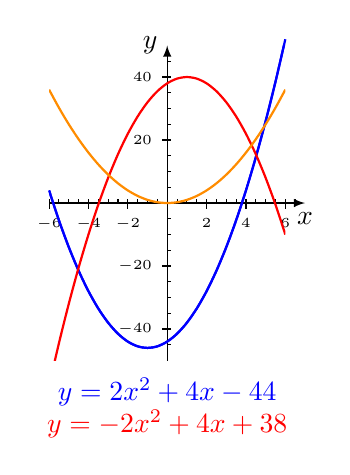
\begin{tikzpicture}[x=2.5mm,y=0.4mm,>=latex]
        \draw[thin,black,->] (-6,0) -- (7,0) node[below] {$x$};
        \draw[thin,black,->] (0,-50) -- (0,50) node[left] {$y$};
        % ticks:
        \foreach \x in {-6,-4,-2,2,4,6}
        {
          \draw[thin,black] (\x,0) -- (\x,-2pt) node[below] {$\scriptscriptstyle\x$};
        }
        \foreach \x in {-6,-5.5,...,6.5}
        {
          \draw[thin,black] (\x,0) -- (\x,1.5pt);
        }
        \foreach \y in {-40,-20,20,40}
        {
          \draw[thin,black] (0,\y) -- (-2pt,\y) node[left] {$\scriptscriptstyle\y$};
        }
        \foreach \y in {-45,-40,...,45}
        {
          \draw[thin,black] (0,\y) -- (1.5pt,\y);
        }
        \draw[thick,blue,domain=-6:6,smooth] plot (\x,{2*(\x)^2+4*\x-44});
        % graphs:
        \begin{scope}
          \clip (-6,-50) rectangle (6,50);
          \draw[thick,blue,domain=-6:6,smooth] plot (\x,{2*(\x)^2+4*\x-44});
          \draw[thick,red,domain=-6:6,smooth] plot (\x,{-2*(\x)^2+4*\x+38});
          \uncover<2->{%
            \draw[thick,orange!90!yellow,domain=-6:6,smooth] plot (\x,{(\x)^2});
          }
        \end{scope}
        % labels:
        \node[blue] at (0,-60) {$y=2x^2+4x-44$};
        \node[red] at (0,-70) {$y=-2x^2+4x+38$};
      \end{tikzpicture}
    \end{center}
  \end{minipage}
  \hfill
  \begin{minipage}{0.5\linewidth}
    \begin{itemize}
    \item $y=ax^2+bx+c$
    \item Bowl-shaped:
      \begin{itemize}
      \item[\red$\star$] Opens up if $a>0$
      \item[\red$\star$] Opens down if $a<0$
      \end{itemize}
    \item Model curve: $y=x^2$ \\
      \uncover<2->{\fbox{\color{orange!90!yellow}Shown here!}}
    \end{itemize}
  \end{minipage}
  \vspace*{2in}

}

\frame{
  \frametitle{Sketching some simple graphs}


  It's useful to be able to sketch\ldots
  \smallskip

  \alert{(2)\ Cubics}

  \begin{minipage}{0.45\linewidth}
    \begin{center}
      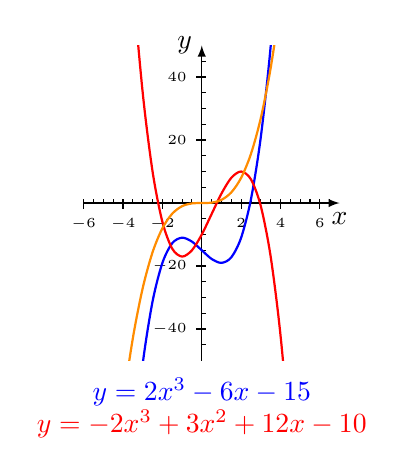
\begin{tikzpicture}[x=2.5mm,y=0.4mm,>=latex]
        \draw[thin,black,->] (-6,0) -- (7,0) node[below] {$x$};
        \draw[thin,black,->] (0,-50) -- (0,50) node[left] {$y$};
        % ticks:
        \foreach \x in {-6,-4,-2,2,4,6}
        {
          \draw[thin,black] (\x,0) -- (\x,-2pt) node[below] {$\scriptscriptstyle\x$};
        }
        \foreach \x in {-6,-5.5,...,6.5}
        {
          \draw[thin,black] (\x,0) -- (\x,1.5pt);
        }
        \foreach \y in {-40,-20,20,40}
        {
          \draw[thin,black] (0,\y) -- (-2pt,\y) node[left] {$\scriptscriptstyle\y$};
        }
        \foreach \y in {-45,-40,...,45}
        {
          \draw[thin,black] (0,\y) -- (1.5pt,\y);
        }
        % graphs:
        \begin{scope}
          \clip (-6,-50) rectangle (6,50);
          \draw[thick,blue,domain=-6:6,smooth] plot (\x,{2*(\x)^3-6*\x-15});
          \draw[thick,red,domain=-6:6,smooth] plot (\x,{-2*(\x)^3+3*(\x)^2+12*\x-10});
          \uncover<2->{%
            \draw[thick,orange!90!yellow,domain=-6:6,smooth] plot (\x,{(\x)^3});
          }
        \end{scope}
        % labels:
        \node[blue] at (0,-60) {$y=2x^3-6x-15$};
        \node[red] at (0,-70) {$y=-2x^3+3x^2+12x-10$};
      \end{tikzpicture}
    \end{center}
  \end{minipage}
  \hfill
  \begin{minipage}{0.5\linewidth}
    \begin{itemize}
    \item $y=ax^3+bx^2+cx+d$
    \item ``S''-shaped:
      \begin{itemize}
      \item[\red$\star$] Goes to $+\infty$ if $a>0$
      \item[\red$\star$] Goes to $-\infty$ if $a<0$
      \end{itemize}
    \item Model curve: $y=x^3$ \\
      \uncover<2->{\fbox{\color{orange!90!yellow}Shown here!}}
    \end{itemize}
  \end{minipage}
  \smallskip
  \uncover<3->{%
    \begin{empheq}[box=\othermathbox]{align*}
      \text{For a polynomial, the {\blue highest power}\ of $x$ {\red dominates}\ when $x$ is big}    
    \end{empheq}
  }
  \vspace*{2in}



}


\section{Computing Derivatives}

\frame{
  \frametitle{The Derivatives of Simple Functions}

  \begin{minipage}{0.45\linewidth}
    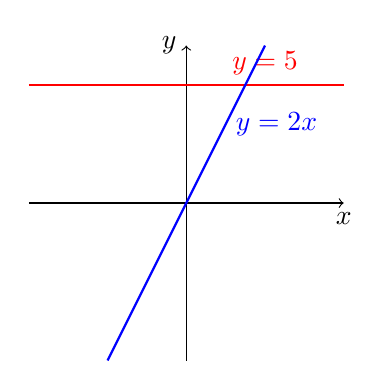
\begin{tikzpicture}
      \draw[thin,black,->] (-2,0) -- (2,0) node[below] {$x$};
      \draw[thin,black,->] (0,-2) -- (0,2) node[left] {$y$};
      \uncover<1-4>{%
        \draw[thick,red] (-2,1.5) -- (2,1.5) node[near end,above] {$y=5$};
      }
      \uncover<5->{%
        \draw[thick,blue] (-1,-2) -- (1,2) node[near end,right] {$y=2x$};
      }
    \end{tikzpicture}
  \end{minipage}
  \hfill
  \begin{minipage}{0.52\linewidth}
    The derivative of a constant is\only<1>{\ldots?}%
    \uncover<2->{%
      \ zero because:
       \begin{itemize}
       \item {\red$\text{derivative} = \text{rate of change}$}
       \item {\red constants don't change}\\[0.5em]
         \uncover<3->{%
       \item {\blue$\text{derivative} = \text{slope}$}
       \item {\blue$\text{slope} = 0$}
         }
       \end{itemize}
      \uncover<4->{So $\dfrac{d}{dx} \big( 5 \big) = 0$}
     }
  \end{minipage}
  \medskip

  \uncover<5->{%
    The derivative of a straight line is\only<5>{\ldots?}}\only<6->{%
    \ its slope because}
  \uncover<6->{%
    \begin{itemize}
    \item {\blue$\text{derivative} = \text{slope}$}
    \end{itemize}
  }
  \uncover<7->{So $\dfrac{d}{dx}\big(2x\big) = 2$}

}


\frame{
  \frametitle{Meaning of Derivatives}

  \begin{minipage}{0.45\linewidth}
    \begin{empheq}[box=\othermathbox]{align*}
      \Large%
      \frac{d}{dx}\left( x^2\right) = 2x      
    \end{empheq}
    % \vspace{.1in}

    What this {\blue means}
    %% \vspace{.1in}

    \begin{empheq}[box=\othermathbox]{align*}
      \text{The {\red slope} of the graph\ }\\
      \text{of ${\blue y=x^2}$ at $x={\red a}$ is $2{\red a}$}
    \end{empheq}
  \end{minipage}
  \hspace*{0.25in}
  \begin{minipage}{0.45\linewidth}
    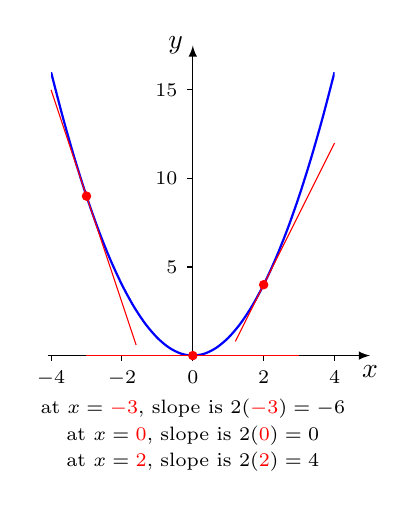
\begin{tikzpicture}[x=4.5mm,y=2.25mm,>=latex]
      \draw[thin,black,->] (-4.1,0) -- (5,0) node[below] {$x$};
      \draw[thin,black,->] (0,0) -- (0,17.5) node[left] {$y$};
      % ticks:
      \foreach \x in {-4,-2,0,2,4}
      {
        \draw[thin,black] (\x,0) -- (\x,-2pt) node[below] {$\scriptstyle\x$};
      }
      \foreach \y in {5,10,15}
      {
        \draw[thin,black] (0,\y) -- (-2pt,\y) node[left] {$\scriptstyle\y$};
      }
      \begin{scope}
        \clip (-4,0) rectangle (4,16);
        \draw[blue,thick,domain=-4:4,smooth] plot (\x,{(\x)^2});
      \end{scope}
      \uncover<2>{%
        \node at (0,-3) {$\scriptstyle\text{at $x={\red-3}$, slope is $2({\red-3})=-6$}$};
        % tangent line is y-9=-6(x+3) or y=-6x-9
        \draw[thin,red,domain=-4:-1.6] plot (\x,{-6*\x - 9});
        \filldraw[red] (-3,9) circle (1.5pt);
      };
      \uncover<3>{%
        \node at (0,-4.5) {$\scriptstyle\text{at $x={\red0}$, slope is $2({\red0})=0$}$};
        % tangent line is y=0
        \draw[thin,red] (-3,0) -- (3,0);
        \filldraw[red] (0,0) circle (1.5pt);
      };
      \uncover<4->{%
        \node at (0,-6) {$\scriptstyle\text{at $x={\red2}$, slope is $2({\red2})=4$}$};
        % tangent line is y-4=4(x-2) or y=4x-4
        \draw[thin,red,domain=1.2:4] plot (\x,{4*\x - 4});
        \filldraw[red] (2,4) circle (1.5pt);
      };
    \end{tikzpicture}
  \end{minipage}
  % \gap

  \uncover<5->{%
    \begin{empheq}[box=\othermathbox]{align*}
      \text{derivative}
      = \text{rate of change}
      = \text{slope of graph}
      = \text{slope of tangent line}
    \end{empheq}
  }



}



\frame{
  \frametitle{General Rule:}

  \begin{minipage}{0.45\linewidth}
    \begin{align*}
      \frac{d}{dx}\left(x^{\red 2}\right) & = {\red 2}x\\
      \frac{d}{dx}\left(x^{\red 3}\right) & = {\red 3}x^{\blue 2}\\
      \frac{d}{dx}\left(x^{\red 4}\right) & = {\red 4}x^{\blue 3}
    \end{align*}
  \end{minipage}
  \begin{minipage}{0.45\linewidth}
    \uncover<2->{%
      \begin{empheq}[box=\othermathbox]{align*}
        \frac{d}{dx}\left(x^{\red n}\right) & = {\red n}x^{\blue n-1}
      \end{empheq}
    }
  \end{minipage}
  \smallskip
  
  \uncover<3->{%
    The {\red exponent} comes out front. Then {\blue subtract} one
    from exponent.
  }

  \uncover<4->{\alert{Examples:}}
  \pause\pause\pause\pause

  {\red(1)} $\dfrac{d}{dx}\left( x^{\red 7}\right) = $
  \begin{center}
    A$ = 7x^7$
    \quad 
    B$ = 6x^6$
    \quad 
    C$ = 6x^7$
    \quad 
    D$ = 7x^6$
    \quad 
    E$ = 0$
    \quad
    \pause
    \fbox{D}
  \end{center}

  {\red(2)} $\dfrac{d}{dx}\left( x^{\red -3}\right) = $
  \begin{center}
    A$ = 3x^{-2}$
    \quad 
    B$ = -3x^{-2}$
    \quad 
    C$ = -2x^{-4}$
    \quad 
    D$ = -3x^{-4}$
    \quad
    \pause
    \fbox{D}
  \end{center}
}

\frame{
  \frametitle{More Examples}
  \begin{empheq}[box=\othermathbox]{align*}
    \frac{d}{dx}\left(x^{\red n}\right) & = {\red n}x^{\blue n-1}
  \end{empheq}

  {\red(3)} $\dfrac{d}{dx}\left( x^{\red 1/2}\right) = $
  \begin{center}
    A$ = \frac{1}{2}x^{1/2}$
    \quad 
    B$ = -\frac{1}{2}x^{-1/2}$
    \quad 
    C$ =  \frac{1}{2}x^{-1/2}$
    \quad
    \pause
    \fbox{C}
  \end{center}
  \pause

  \alert{Rule:}\ {\red ALWAYS}\  {\blue re}write {\blue the
    thing} you want derivative of  as $x^{\red n}$
  \pause\smallskip

  {\red(4)} $\dfrac{d}{dx}\left( {\frac{1}{x^3}}\right) = $
  \begin{center}
    A$ = \frac{1}{3x^2}$
    \quad 
    B$ = -3x^{-2}$
    \quad 
    C$ = -3x^{-4}$
    \quad
    \pause
    \fbox{C}
  \end{center}
  \pause

  {\red(5)} $\dfrac{d}{dx}\left({\sqrt{x}}\right) = $
  \begin{center}
    A$ =-\frac{1}{2}\sqrt{x}$
    \quad 
    B$ = \frac{1}{2}{x}^{-1/2}$
    \quad 
    C$ =  -\frac{1}{2}{x}^{-1/2}$
    \quad
    \pause
    \fbox{B}
  \end{center}


}

\frame{
  \frametitle{Polynomials}

  \begin{equation*}
    \frac{d}{dx}\left(4x^{\red 5}+7x^{\blue 2}-{\purple 5x}+{\bluegreen 7}\right)
    = 4({\red 5})x^{\red 4}+7({\blue 2})x^{\blue 1} - {\purple 5}+{\bluegreen 0}
  \end{equation*}
  \pause

  \alert{Special cases}
  \begin{itemize}
  \item $\dfrac{d}{dx}\left( {\purple -5 x} \right)={\purple -5}$
    \pause

  \item $\dfrac{d}{dx}\left( {\bluegreen 7} \right)={\bluegreen 0}$
    \pause

  \end{itemize}
  \gap

  \alert{Question:}\ $\displaystyle\frac{d}{dx}\left(3x^{\red 4}+9x^{\blue 3}+{\bluegreen 7}\right)=$?
  \begin{center}
    A$ = \text{I have an answer}$
    \qquad 
    B$ = \text{I am working on it}$
    \qquad 
    C$ = \text{Help!}$
    \pause
  \end{center}

  \alert{Answer:}\ $12x^3+27x^2$
  \begin{center}
    A$ = \text{I got it}$
    \qquad 
    B$ = \text{I nearly got it}$
    \qquad 
    C$ = \text{I want my mommy!}$
  \end{center}


}

\section{Meaning \& Applications}

\frame{
  \frametitle{The Meanings of Derivatives}

  The derivative of $f(x)=x^2+3x+1$ is $f'(x)=\frac{df}{dx}=2x+3$.
  This means:
  \begin{itemize}
  \item[\nb] This is the {\red slope}\ of the graph $y=x^2+3x+1$ at the
    point ${\blue x}$
    \pause

  \item[\nb] It is the {\red instantaneous rate of change}\ of
    $f({\blue x})$ at ${\blue x}$.
  \pause

  \end{itemize}
  \gap

  That $f'(2) = 7$ means:
  \begin{itemize}
  \item[\nb] The {\red slope}\ of the graph $y=f({\blue x})$ at $x={\blue 2}$
    is ${\green 7}$.
    \pause

  \item[\nb] The {\red slope of the tangent line}\ to the graph at ${\blue
      x}={\blue 2}$ is ${\green 7}$.
    \pause

  \item[\nb] The {\red instantaneous rate of change}\ of $f(x)$ at
    ${\blue x}={\blue 2}$ is ${\green 7}$.
    \pause

  \item[\nb] At ${\blue x}={\blue 2}$ the output (value of $f({\blue
      x})$) changes ${\red 7}$ times as fast as the {\blue input}
    (value of ({\blue x})).
    \pause
    
  \item[\nb]  $\Delta f\approx {\red 7}\Delta {\blue x}$ near
    ${\blue x}={\blue 2}$.
    \pause

  \item[\nb] $f({\blue 2}+\Delta {\blue x})\approx f({\blue 2})+{\red 7}\Delta x$.
  \end{itemize}
 

}

\frame{
  \frametitle{Applications}

  {\red(1)} What is the slope of the graph $y= 3x^2-7x+5$ at $x=1$?
  \begin{center}
    A$=-2$
    \quad 
    B$=-1$
    \quad 
    C$=0$
    \quad 
    D$=1$
    \quad 
    E$=2$
    \pause
    \quad
    \fbox{B}
  \end{center}
  \gap

  {\red(2)} What is the instantaneous rate of change of $f(x)=x^3-2x+3$ at $x=1$?
  \begin{center}
    A$=-2$
    \quad 
    B$=-1$
    \quad 
    C$=0$
    \quad 
    D$=1$
    \quad 
    E$=2$
    \pause
    \quad
    \fbox{D}
  \end{center}
  \gap

  {\red(3)}\ After $t$ seconds a hamster on a skate board is $4t^2+2t$
  cm from the origin on the $x$-axis. What is the exact speed of the
  hamster (in cm/sec) after $2$ seconds?
  \begin{center}
    A$=10$
    \quad 
    B$ = 16$
    \quad 
    C$ = 18$
    \quad 
    D$ = 20$
    \quad 
    E$ =14$
    \pause
    \quad
    \fbox{C}
  \end{center}

}

\frame{
  \frametitle{Why This Works (\S8.9)}
  \begin{empheq}[box=\othermathbox]{align*}
    \frac{d}{dx}\left(x^{\red n}\right) & = {\red n}x^{\blue n-1}
  \end{empheq}

  \uncover<2->{%
    \alert{Example: $n=3$:}\ Calculate the average rate of change of
    $x^3$ between ${\blue x}$ and $x+\text{{\red\only<3->{$h$}\only<2>{$\Delta
          x$}}}$ then take limit as
    {\red\only<3->{$h$}\only<2>{$\Delta x$}}$\to 0$.
  }

  \begin{align*}
    \uncover<4->{%
    \left(
    \begin{array}{c} 
      \text{average rate}\\ 
      \text{of change between}\\ 
      \text{$x$ and $x+{\red h}$}
    \end{array}
    \right)     
    }
    & \uncover<5->{ = \frac{({ {x}+{\red h}})^{3}-{ {x}^{ 3}}}{({x}+{\red h})-{ x}}}\\
    % & = \frac{({\green x}^3+3{\green x}^2{\purple h}+3{\green x}{\purple h}^2+{\purple h}^3)-{\blue {\green x}^3}}{{\purple h}}\\ 
    % \pause
    % & = \frac{3{\green x}^2{\purple h}+3{\green x}{\purple h}^2+{\red h}^3}{{\purple h}}\\ 
    % \pause
    & \uncover<6->{= 3x^2+3x{\red h}+{\red h}^2}
  \end{align*}
  \uncover<7->{%
    Limit as ${\red h}\to0$ is \fbox{$3x^2$}
  }
  \gap 
  
  \uncover<8->{%
    A similar calculation works for $x^{\red n}$ for any ${\red n}$.
  }
}


\frame{
  \frametitle{More Applications}

  What is the equation of the tangent line at $x={1}$ to the
  graph of  $y=x^3-x+4$?  The tangent line is $y=\ldots$?
  \begin{center}
    A$ = x+3$
    \quad 
    B$ = 3x+1$
    \quad 
    C$ = 2x-2$
    \quad 
    D$=2x+2$
    \quad 
    E$=6x-2$
    \uncover<2->{\qquad\fbox{D}}
  \end{center}
  \uncover<3->{%
    Here's a picture:

    \begin{center}
      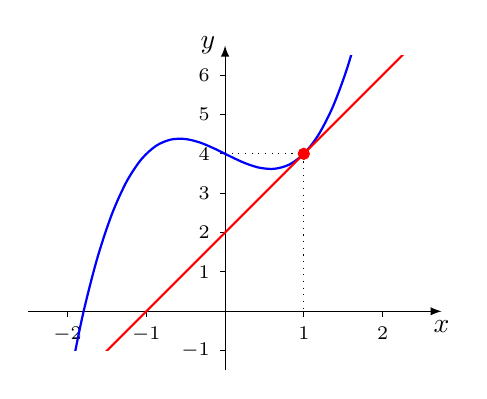
\begin{tikzpicture}[x=10mm,y=5mm,>=latex]
        \draw[thin,black,->] (-2.5,0) -- (2.75,0) node[below] {$x$};
        \draw[thin,black,->] (0,-1.5) -- (0,6.75) node[left] {$y$};
        % ticks:
        \foreach \x in {-2,-1,1,2}
        {
          \draw[thin,black] (\x,0) -- (\x,-2pt) node[below] {$\scriptstyle\x$};
        }
        \foreach \y in {-1,1,2,3,4,5,6}
        {
          \draw[thin,black] (0,\y) -- (-2pt,\y) node[left] {$\scriptstyle\y$};
        }
        \draw[thin,black,dotted] (0,4) -- (1,4) -- (1,0);
        \begin{scope}
          \clip (-2,-1) rectangle (2.5,6.5);
          \draw[thick,blue,domain=-2:2.5,smooth] plot (\x,{(\x)^3-\x+4});
        \end{scope}
        \begin{scope}
          \clip (-2,-1) rectangle (2.5,6.5);
          \draw[thick,red,domain=-2:2.5,smooth] plot (\x,{2*\x+2});
        \end{scope}
        \filldraw[red] (1,4) circle (2pt);
      \end{tikzpicture}
    \end{center}
  }
}

\frame{
  \frametitle{Another Example}

  The temperature in an oven after $t$ minutes is
  $50+t^3\ {}^{\circ}\,\text{F}$.  How quickly is the temperature
  rising after $2$ minutes?
  \begin{center}
    A$=58$
    \quad 
    B$ = 3$
    \quad 
    C$ = 12$
    \quad 
    D$ = 50$
    \quad 
    E$ = 8$
    \pause
    \quad
    \fbox{C}
  \end{center}
}

\end{document}

\frame{
  \frametitle{A Warning!}
  \fbox{\parbox[b]{110mm}{{\red WARNING} 
      \begin{equation*}
        \frac{d}{dx}\left(f(x)g(x)\right) {\blue\ne}\frac{df}{dx}\frac{dg}{dx}
      \end{equation*}
      \gap
      \alert{Example:} \quad $5x^4=\frac{d}{dx}\left(x^5\right)=\frac{d}{dx}\left(x^2\cdot x^3\right){\red\ne}(2x)(3x^2)=6x^3$}}
  \gap

  \alert{Example:} Find derivative of $(x+1)(2x+3)$
  \vspace*{1in}
}


\frame{
  \frametitle{An Example For You}

  \alert{Question:}\ $\displaystyle\frac{d}{dx}\left((x^2+1)(x^3+1)\right)=$?
  \begin{center}
    A$=6x^3$
    \quad 
    B$ = 5x^4+3x^2+2x$
    \quad 
    C$ = x^5+x^3+x^2+1$
    \quad 
    D$ = \text{Other}$
  \end{center}
  \bigskip
  \pause

  \alert{Answer:}\ \fbox{B}

  \vspace*{2in}

}




\frame{
  \frametitle{Once upon a time\ldots} 

  There was a happy math professor and he told his
  happy students: ``When you work out {\blue derivatives} {\red ALWAYS}
  write the $\frac{d}{dx}$ part so you write something like
$$\frac{d}{dx}\left(3x^2+5x+2\right) = 6x+5$$
and you never-ever-ever write\\
\fbox{$3x^2+5x+2\qquad 6x+5$} or even worse \fbox{$3x^2+5x+2=6x+5$}

Because if you don't do as I say I will become a  sad   math professor and you will repeat this class.''

}



\frame{

$f(x)=\sqrt{x}.$ What is $f'(16) ?$\\
$A=\frac{1}{2}\quad B=\frac{1}{4}\quad C=\frac{1}{8}\quad D=\frac{1}{16}\quad E = \frac{1}{32}$\pause\quad\fbox{\blue C}\\
\ \ $\because f'(x)=\frac{1}{2}x^{-1/2}\ so\ f'(16)=\left(\frac{1}{2}\right)(16)^{-1/2}=\left(\frac{1}{2}\right)\frac{1}{\sqrt{16}}=\frac{1}{8}$

\gap
A circle is expanding so that after $R$ seconds it has radius $R$ cm.\\
What is the rate of increase of area inside the circle after 2 seconds ?\\
$A=4\pi \quad B = 2\pi R^2\quad C =2\quad D = 2\pi R\quad E = \pi R^2 $\pause\quad\fbox{\blue A}

\gap $A(R)=$ area inside circle of radius $R$\\
rate of increase of area
= derivative
= $\frac{d}{dR}\left(\pi R^2\right)=2\pi R$\\
So rate of increase of area when $R=2$ is $2\pi(2)=4\pi$

\gap What is the $x$-coordinate of the point on the graph of $y=4x^2-3x+7$ where the graph has slope ${\purple 13}$ ?\\
$A=0\quad B=1\quad C=2\quad D=3\quad E=4$\pause\quad\fbox{\blue C}

slope
= derivative\\
$=\frac{d}{dx}\left(4x^2-3x+7\right)=8x-3$\\
Want to know when this equals ${\purple 13}$\\
Solve ${\purple 13}=8x-3$ get $8x=13+3=16$ so \fbox{$x=2$}

}


\frame{


\gap
{\blue Once upon a time.....} There was a happy math professor {\red \Huge\Smiley} and he told his happy students: "When you work out {\blue derivatives} {\red ALWAYS} write the $\frac{d}{dx}$ part
so you write something like
$$\frac{d}{dx}\left(3x^2+5x+2\right) = 6x+5$$
and you never-ever-ever write\\
\fbox{$3x^2+5x+2\qquad 6x+5$} or even worse \fbox{$3x^2+5x+2=6x+5$}

Because if you don't do as I say I will become a  sad   math professor and you will repeat this class {\blue \Huge\Frowny}

}

\frame{

$f(x)=\sqrt{x}.$ What is $f'(16) ?$\\
$A=\frac{1}{2}\quad B=\frac{1}{4}\quad C=\frac{1}{8}\quad D=\frac{1}{16}\quad E = \frac{1}{32}$\pause\quad\fbox{\blue C}\\
\ \ $\because f'(x)=\frac{1}{2}x^{-1/2}\ so\ f'(16)=\left(\frac{1}{2}\right)(16)^{-1/2}=\left(\frac{1}{2}\right)\frac{1}{\sqrt{16}}=\frac{1}{8}$

\gap
A circle is expanding so that after $R$ seconds it has radius $R$ cm.\\
What is the rate of increase of area inside the circle after 2 seconds ?\\
$A=4\pi \quad B = 2\pi R^2\quad C =2\quad D = 2\pi R\quad E = \pi R^2 $\pause\quad\fbox{\blue A}

\gap $A(R)=$ area inside circle of radius $R$\\
rate of increase of area
= derivative
= $\frac{d}{dR}\left(\pi R^2\right)=2\pi R$\\
So rate of increase of area when $R=2$ is $2\pi(2)=4\pi$

\gap What is the $x$-coordinate of the point on the graph of $y=4x^2-3x+7$ where the graph has slope ${\purple 13}$ ?\\
$A=0\quad B=1\quad C=2\quad D=3\quad E=4$\pause\quad\fbox{\blue C}

slope
= derivative\\
$=\frac{d}{dx}\left(4x^2-3x+7\right)=8x-3$\\
Want to know when this equals ${\purple 13}$\\
Solve ${\purple 13}=8x-3$ get $8x=13+3=16$ so \fbox{$x=2$}

}



\frame{


\gap
{\blue Once upon a time.....} There was a happy math professor {\red \Huge\Smiley} and he told his happy students: "When you work out {\blue derivatives} {\red ALWAYS} write the $\frac{d}{dx}$ part
so you write something like
$$\frac{d}{dx}\left(3x^2+5x+2\right) = 6x+5$$
and you never-ever-ever write\\
\fbox{$3x^2+5x+2\qquad 6x+5$} or even worse \fbox{$3x^2+5x+2=6x+5$}

Because if you don't do as I say I will become a  sad   math professor and you will repeat this class {\blue \Huge\Frowny}

}

\frame{

$f(x)=\sqrt{x}.$ What is $f'(16) ?$\\
$A=\frac{1}{2}\quad B=\frac{1}{4}\quad C=\frac{1}{8}\quad D=\frac{1}{16}\quad E = \frac{1}{32}$\pause\quad\fbox{\blue C}\\
\ \ $\because f'(x)=\frac{1}{2}x^{-1/2}\ so\ f'(16)=\left(\frac{1}{2}\right)(16)^{-1/2}=\left(\frac{1}{2}\right)\frac{1}{\sqrt{16}}=\frac{1}{8}$

\gap
A circle is expanding so that after $R$ seconds it has radius $R$ cm.\\
What is the rate of increase of area inside the circle after 2 seconds ?\\
$A=4\pi \quad B = 2\pi R^2\quad C =2\quad D = 2\pi R\quad E = \pi R^2 $\pause\quad\fbox{\blue A}

\gap $A(R)=$ area inside circle of radius $R$\\
rate of increase of area
= derivative
= $\frac{d}{dR}\left(\pi R^2\right)=2\pi R$\\
So rate of increase of area when $R=2$ is $2\pi(2)=4\pi$

\gap What is the $x$-coordinate of the point on the graph of $y=4x^2-3x+7$ where the graph has slope ${\purple 13}$ ?\\
$A=0\quad B=1\quad C=2\quad D=3\quad E=4$\pause\quad\fbox{\blue C}

slope
= derivative\\
$=\frac{d}{dx}\left(4x^2-3x+7\right)=8x-3$\\
Want to know when this equals ${\purple 13}$\\
Solve ${\purple 13}=8x-3$ get $8x=13+3=16$ so \fbox{$x=2$}

}





\end{document}